\documentclass[]{lnudissertation}
\sloppy

% ============================================================
% 1. ENCODING, LANGUAGE, BIBLIOGRAPHY
% ============================================================
\usepackage[T1]{fontenc}
\usepackage[utf8]{inputenc}
\usepackage[swedish,english]{babel}
\usepackage[
  backend=biber,
  style=numeric,
  maxcitenames=1,
  maxbibnames=99
]{biblatex}
\addbibresource{refs.bib}

%% 1. ACM (Association for Computing Machinery)
\RequirePackage{libertine}
\RequirePackage[libertine]{newtxmath}

%% 2. IEEE (Institute of Electrical and Electronics Engineers)
%% Style: Times New Roman clone (Standard, space-efficient engineering look)
% \RequirePackage{newtxtext}
% \RequirePackage[varg]{newtxmath}  % varg gives an italic 'g' preferred by IEEE

%% 3. JSS (Journal of Statistical Software) / AMS / SIAM
%% Style: Latin Modern (The definitive high-quality classical LaTeX layout)
% \RequirePackage{lmodern}


% ============================================================
% 3. TEXT FORMATTING AND TYPOGRAPHY
% ============================================================
\usepackage{enumerate}
\usepackage{enumitem}
\usepackage{csquotes}
\usepackage{setspace}
\setstretch{1.03}
% \spaceskip=1 \fontdimen2\font plus 1 \fontdimen2\font minus 1\fontdimen2\font
% \DeclareUnicodeCharacter{0302}{\^{}}

% ============================================================
% 4. FIGURES, TABLES, LAYOUT
% ============================================================
\usepackage{graphicx}
\usepackage{caption}
\usepackage{booktabs}
\usepackage{siunitx}
\usepackage{adjustbox}
\usepackage{array}
\usepackage{multirow}
\usepackage[most]{tcolorbox}
\usepackage{tabularx}
\usepackage{threeparttable}
% ============================================================
% 5. DOCUMENT STRUCTURE / NAVIGATION
% ============================================================
\usepackage{verbatim}   % multi-line comments
\usepackage{appendix}
\renewcommand{\appendixtocname}{Appended Publications}
\usepackage[framemethod=TikZ]{mdframed} % required: GrayBox ("Answer to RQx") boxes used throughout all paper chapters

% ============================================================
% 6. STAMPS, OVERLAYS, POSITIONING
% ============================================================
\usepackage[absolute,overlay]{textpos} % required by \draftstamp / \overlaypagenote
% ============================================================
% 7. HYPERLINKS AND URLS
% ============================================================
\usepackage{url}
\urlstyle{acsstyle}
\usepackage{xurl}

\makeatother

\hypersetup{
    hidelinks, % no boxes around hyperlinks
    pdfinfo={
        Title={[Graph Representation Learning for Software Architecture Recovery]},
        Author={Rakhshanda Jabeen},
        Subject={PhD Dissertation},
        Keywords={Software Architecture Recovery; Code-to-Architecture Mapping; Graph Neural Networks; Representation Learning; Software Engineering},
    }
}
% ============================================================
% 8. CUSTOM COMMANDS -- GENERAL HELPERS
% ============================================================
\newtcolorbox{GrayBox}[2][]{%
  enhanced,
  width=\textwidth,
  colback=gray!5,
  colframe=black!60,
  % coltitle=black,
  arc=0.5mm,
  boxrule=0.7pt,
  left=0.5ex,
  right=0.5ex,
  top=1ex,
  bottom=1ex,
  before skip=3ex,
  after skip=3ex,
  title=#2,
  #1
}

% ============================================================
% 9. CUSTOM COMMANDS -- THESIS-SPECIFIC (paper cross-referencing)
% ============================================================
\newcommand{\citepaper}[1]{Paper~\ref{app:publ-#1}}
\newcommand{\citepaperp}[1]{(\citepaper{#1})}
\newcommand{\citearticle}[1]{Article~\ref{app:publ-#1}}
\newcommand{\citearticlep}[1]{(\citearticle{#1})}

% ============================================================
% 10. CUSTOM COMMANDS -- RECURRING METRIC / TERM SHORTHANDS
% ============================================================
\newcommand{\cc}{C2C\textsubscript{cvg}}
\newcommand{\tmq}{TMQ\textsubscript{norm}}
%----------------------------------------------------------------------------------------------------
%------------------------HERE STARTS THE PRINTING --------------------------------
%----------------------------------------------------------------------------------------------------
\begin{document}
\frontmatter
% chapters/00_front-matter-lud.tex
% Working title page only.
% LNU Press will normally provide the final camera-ready title page.

\thispagestyle{empty}

\begin{center}

\vspace*{4.5cm}

{\normalsize Rakhshanda Jabeen\par}

\vspace{1.5cm}

{\Large\bfseries
Representing Architectural Evidence in Software Systems: A Graph Learning Approach\par}

\vspace{2cm}

{\normalsize
Doctoral Dissertation\par
\vspace{0.2cm}
Computer Science / Software Technology\par
\vspace{0.4cm}
2026\par}

\vfill


\includegraphics[scale=0.2]{images/lnu.pdf}

\end{center}

\cleardoublepage
\null
\vfill
\noindent
\begin{minipage}{\textwidth}%
\raggedleft%
%\emph{Dedicated to\ldots}%
\emph{To my mother.}
\end{minipage}%
\vfill

\cleardoublepage
\vspace*{\stretch{1}}
\begin{center}
{\arabicfont\Large \beginR وَفَوْقَ كُلِّ ذِي عِلْمٍ عَلِيمٌ ۝٧٦\endR}

\vspace{2em}

{\large\itshape \enquote{And above every possessor of knowledge is \textbf{one} more knowing.}}

\vspace{1em}

{\small Quran, Surah Yusuf (12:76)}
\end{center}
\vspace*{\stretch{1.5}}
% 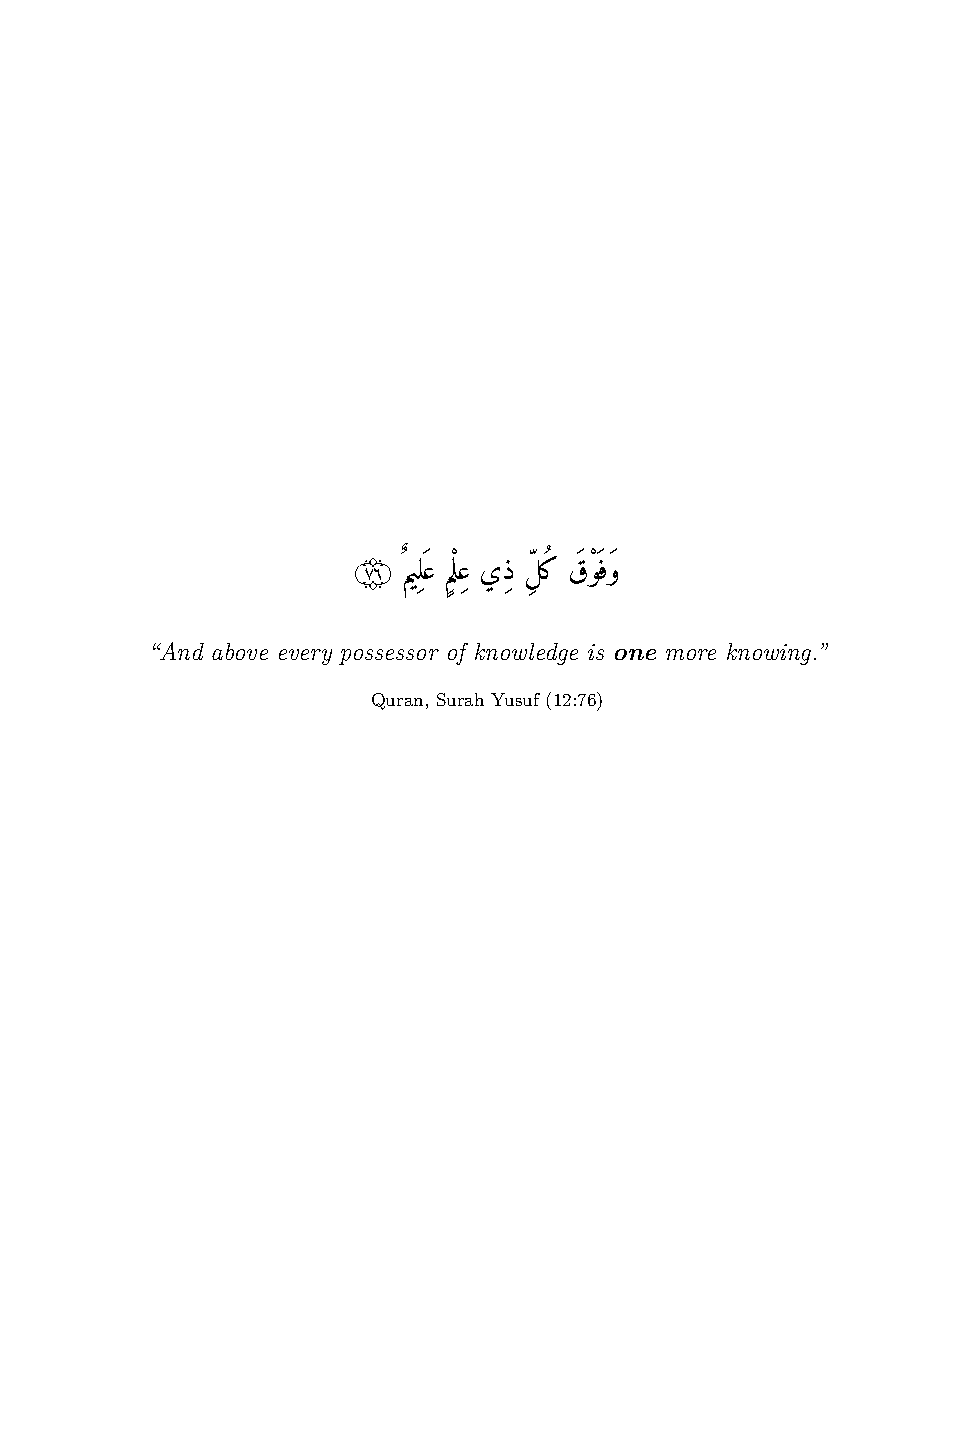
\includepdf[pages=1,pagecommand={\thispagestyle{plain}}]{images/arabic_verse.pdf}
\cleardoublepage

\begin{abstract}
{\small
Software architecture documentation is often missing, incomplete, or outdated, making it unclear which source files implement which architectural modules. Software architecture recovery infers a modular decomposition from the implementation, while code-to-architecture mapping assigns files to known modules using a partial mapping. Both tasks can use dependencies, folder structure, and source code, but existing methods often rely on individual sources or predefined combinations. It remains unclear what each source contributes and when propagating information between connected files helps rather than mixes evidence from different modules.

The research uses open-source Java, C, and C++ systems with published reference decompositions. Recovery studies examine learning objectives, graph construction, and information sources, while mapping studies investigate representations, graph-based propagation, and iterative self-training.

For architecture recovery, learned representations achieve agreement with reference architectures comparable to or better than the evaluated baselines. In the evaluated configurations, reconstruction generally outperforms contrastive learning, while random walks and diffusion capture structural information beyond direct dependencies. However, combining structural, lexical, and folder information can improve agreement with reference architectures while producing modules with weaker dependency cohesion than those obtained from dependency-based random-walk embeddings.

For code-to-architecture mapping, neural classifiers outperform a Naive Bayes baseline. A graph attention network outperforms a graph-free classifier on most systems, although gains vary by system and configuration. Folder information produces the largest and most consistent improvements, but higher accuracy can coincide with misclassifications of files that a simple directory rule assigns correctly. Representations that encode dependencies generally outperform lexical ones, and dependency-guided fine-tuning improves contextual representations. 

However, strong graph-model performance does not by itself demonstrate a benefit from additional message passing. Controlled experiments show that propagating dependency information can reduce performance for some predictors compared with matched models without cross-file messages. Changes to graph construction, propagation methods, or learning settings can reduce these losses or lead to improvements.

Together, these findings show that the usefulness of architectural information depends not only on what is available, but also on how it is represented, combined, and used.

}

\bigskip
\vfill
\noindent
\textbf{Keywords:}
Software Architecture, Software Architecture Recovery, Representation Learning, Graph Neural Networks, Graph Autoencoders

\end{abstract}
\cleardoublepage



\begin{acknowledgments}
\null

I want to thank myself :)


%% With the null, we avoid the space when starting a new paragraph, if necessary
%\null
\bigskip
\vfill
\noindent V\"axj\"o, Sweden\\
\noindent 2023\\
\bigskip

\end{acknowledgments}
\cleardoublepage


\renewcommand\contentsname{Table of Contents}
\setcounter{tocdepth}{1}
\phantomsection
\addcontentsline{toc}{chapter}{\contentsname{}}
\tableofcontents
\cleardoublepage
\phantomsection
\addcontentsline{toc}{chapter}{\listfigurename{}}
\listoffigures
\cleardoublepage
\phantomsection
\addcontentsline{toc}{chapter}{\listtablename{}}
\listoftables
\cleardoublepage
\chapter*{List of Abbreviations}
\begin{description}
\item[A2A] Architecture-to-architecture
\item[ARI] Adjusted Rand index
\item[AST] Abstract Syntax Tree
\item[BoW] Bag-of-words
\item[C2A] Code-to-architecture
\item[DGI] Deep Graph Infomax
\item[GAE] Graph autoencoder
\item[GAT] Graph attention network
\item[GCN] Graph convolutional network
\item[GDC] Graph diffusion convolution
\item[GNN] Graph Neural network
\item[HGT] Heterogeneous Graph Transformer
\item[LPE] Laplacian positional encoding
\item[MLP] Multi layer perceptron
\item[MoJoFM] Move and join operations
\item[MQ] Modularization quality
\item[N2V] Node2Vec
\item[PPR] Personalized PageRank
\item[SAR] Software architecture recovery
\item[SDG] Software dependency graph
\item[TurboMQ] Turbo modularization quality
\item[VGAE] Variational graph autoencoder
\item[W2V] Word2Vec
\end{description}

%% The list of listings is not tested!!
%% Add the listings package in case it is needed, too
%\lstlistoflistings
%% Add the list of publications
\cleardoublepage
\chapter*{List of Publications}
\addcontentsline{toc}{chapter}{List of Publications}
\markboth{List of Publications}{List of Publications}

\noindent This dissertation is based on the following publications. I contributed to all stages of the work as lead author.

\begin{enumerate}[leftmargin=*,label=\Roman*.,itemsep=1.2em,topsep=0pt]
    \item\myfullcite{arl_2026}~(page~\pageref{app:publ-arl_2026}).
    \item\myfullcite{gaer}~(page~\pageref{app:publ-gaer}).
    \item\myfullcite{c2a_mapping}~(page~\pageref{app:publ-c2a_mapping}).
    \item\myfullcite{structsar}~(page~\pageref{app:publ-structsar}).
    \item\myfullcite{hetmap}~(page~\pageref{app:publ-hetmap}).
\end{enumerate}
\cleardoublepage
%------------------------------------------------------------------------
%---------------------HERE STARTS THE THESIS CONTENT---------------------
%------------------------------------------------------------------------
\mainmatter
% ---------------------------------------------------------------------
% CHAPTER 1 — INTRODUCTION
% Job: establish the problem and the single thesis. NO overarching RQs here.
% ---------------------------------------------------------------------
\chapter{Introduction \label{ch:introduction}}

% 1.1 The problem, stated once, concretely.
%   - Architecture drifts/erodes; documentation goes stale; mappings are missing.
%   - SAR and C2A mapping defined and distinguished (recovery = discover the
%     decomposition; mapping = assign entities given partial known architecture).
%   - Cost anchor: expert C2A mapping is ~107 person-hours/system; Chromium took
%     ~2 years. This is the "why automate" evidence, not rhetoric.
\section[Architectural Erosion and Recovery]{Software Architecture Erosion and the Recovery}

% 1.2 Why the obvious approaches are insufficient (motivates the whole thesis).
%   - Dependency-only clustering: "connected by an edge" != "same module".
%   - Hand-tuned fusion (SARIF): fixed weights don't generalize across systems/scale.
%   - The gap: no single signal suffices, and hand-weighting them doesn't either.
\section{Why architectural signal is hard to use}

% 1.3 The thesis statement (the spine). State it plainly:
%   Architectural structure is distributed across several implementation signals
%   (typed dependencies, folder organization, lexical identifiers, member-level
%   detail). Learned graph representations integrate them better than hand-tuned
%   fusion; and recovery is bounded not by the encoder but by whether the target
%   architecture is reflected in the chosen signal and whether the model's reach
%   matches system scale and granularity.
\section{Thesis statement and scope}

% 1.4 Contributions of the thesis as a whole (not per-paper yet).
%   - C1: learned representations beat hand-tuned fusion, most clearly at scale.
%   - C2: isolation of what each signal contributes and where it fails.
%   - C3: the same signals/systems hold across unsupervised recovery AND
%         supervised mapping (the duality that no single paper can claim).
%   - C4: directory structure as a strong architectural proxy, shown by removing it.
\section{Contributions}

% 1.5 Included papers + author roles + a one-line "what each isolates".
\section{Included publications}

% 1.6 Thesis outline (short).
\section{Outline}
% \section{Motivation: Architecture Erosion and the Cost of Technical Debt}
% \label{sec:motivation}

% As software systems evolve through refactoring, feature additions, and ongoing maintenance, the implemented system gradually diverges from its intended architectural design. This architectural drift, or erosion, degrades maintainability, understandability, and long-term evolvability~\cite{bass2012software,de2012controlling}. Static Architecture Conformance Checking (SACC) techniques, such as reflexion modeling, address this problem by comparing implementation-level dependencies against architecture-level relations to identify convergent, divergent, and absent dependencies~\cite{reflexion1, SACCcomparison}. Applying these techniques presupposes that a decomposition of the system into architectural modules is available. In many systems, no such decomposition is documented or maintained, and it must instead be recovered directly from the implementation.
 
% Software Architecture Recovery (SAR) addresses this first problem: inferring a system's modular decomposition from its source code, without assuming that an intended architecture is already known. Recovering an architecture manually is labor-intensive and does not scale; recovering the decomposition of a medium-sized system can require hundreds of hours of expert effort~\cite{garcia2013}. This motivates automated recovery techniques that infer modular structure directly from implementation artifacts such as dependencies, folder organization, and code identifiers.
 
% Recovery, however, is not the only setting in which this problem arises. In many systems, an intended architecture already exists, but the mapping between implementation-level entities and architectural modules is incomplete, outdated, or was never fully documented~\cite{ali2018architecture}. Here, the task is not to discover a decomposition from scratch, but to propagate a small amount of known mapping to the remainder of the system, a problem generally referred to as code-to-architecture (C2A) mapping. Both problems, recovery and mapping, require inferring architectural structure from the same underlying implementation signals, differing primarily in how much architectural knowledge is available as supervision: none, in recovery, and partial, in mapping. Maintaining this mapping is a growing concern as the volume of machine-generated code entering software systems increases, since such code is produced without visibility into a system's module structure~\cite{ehsani2025fastercode,wu2025clones}.
 
% Existing techniques for both problems typically combine multiple implementation signals, such as static dependencies, folder organization, and lexical identifiers, through hand-crafted similarity functions and manually tuned weights~\cite{sarif,sade}. Because dependency patterns and architectural styles differ across systems, such fixed heuristics do not generalize consistently. This motivates a data-driven alternative: learning, rather than hand-specifying, how these signals should be combined and weighted for a given system.

% Every non-trivial software system begins with an intended architecture: a decomposition into modules, layers, or subsystems that encodes the designers' understanding of how responsibilities should be separated and how components should interact. As a system evolves under the pressure of deadlines, changing requirements, and developer turnover, its \emph{implemented} architecture tends to drift away from this intended structure. This phenomenon, known as \textbf{architecture erosion} (or architectural degradation), has been studied extensively in the software engineering literature and is consistently linked to rising maintenance costs, reduced developer productivity, and increased defect rates as systems age~\citep{li2022erosion}.

% The financial framing for this problem was introduced by Ward Cunningham, who coined the \textbf{technical debt} metaphor to describe the trade-off between short-term development speed and long-term maintainability:

% \textit{``Shipping first time code is like going into debt\ldots{} the danger occurs when the debt is not repaid.''}

% \hfill --- \citet{cunningham1992wycash}

% When this debt accumulates specifically at the level of a system's structure, in its module boundaries, layering, and dependency organization, it is termed \textbf{architectural technical debt (ATD)}: design or implementation constructs that are expedient in the short term but make future changes more costly, precisely because they violate or obscure the system's intended decomposition~\citep{kruchten2012technicaldebt,nord2012metric}. The technical debt community formalizes this short-term/long-term trade-off using two further concepts borrowed directly from finance: the \textbf{principal}, the cost of the rework required to bring a system back to a well-architected state, and the \textbf{interest}, the recurring extra cost paid on every subsequent change until that rework happens~\citep{verdecchia2020grounded}. Code-level debt is often locally visible as a "smell" in a single file and can be readily flagged by static analyzers. Architectural debt is different: it lives in the relationships \emph{between} components, is invisible to any single developer working within one module, and tends to be discovered only once its accumulated interest, the extra effort required to make a change that should have been simple, becomes large enough to notice. Existing attempts to make ATD measurable, such as the ATDx index, aggregate violations of a manually curated set of architectural rules into a single score~\citep{verdecchia2020atdx}. That approach is useful, but only as good as the rules an analyst thought to specify in advance. This asymmetry, between the difficulty of \emph{detecting} architectural debt (diffuse, relational, and only partially captured by hand-picked rules) and the ease of \emph{incurring} it, motivates the two complementary problems this dissertation addresses.

% The first problem is a matter of \textbf{diagnosis}: once documentation has gone stale or was never created, how can we recover an accurate, up-to-date picture of a system's actual architecture directly from its code, so that architectural technical debt, and specifically its accumulated \emph{principal}, can even be identified in the first place? The second problem is a matter of \textbf{prevention}: given that a system already has a known, intended decomposition into modules, how can new or previously unclassified code be correctly and consistently placed within it, so that architectural debt stops accumulating and stops charging \emph{interest} on every subsequent change, simply because developers lack automated guidance on where new code belongs? Both problems are, at their core, about recovering or preserving the correspondence between a codebase's structure and its architecture: one after the correspondence has been lost and debt has already accrued, the other before it can be lost, preventing debt from accruing at all. This dissertation studies both, using graph neural network-based representation learning as the common technical vehicle, and treats technical debt as the motivation revisited throughout every subsequent chapter.

% \section{Problem Statement: Two Complementary Architectural Tasks}
% \label{sec:problem-statement}

% We study two related but distinct tasks throughout this body of work.

% \paragraph{Software Architecture Recovery (SAR)} is the \emph{unsupervised} problem of inferring a module-level decomposition of a software system directly from its source code, with no ground-truth structure provided as input. The output is typically a clustering of code entities (files, classes) into architecturally meaningful groups, evaluated against an expert-defined or historically documented "true" decomposition. SAR is the appropriate task when documentation is absent, outdated, or untrustworthy: the diagnostic scenario above.

% \paragraph{Software/Code-to-Architecture Mapping (SC2AM)} is the \emph{semi-supervised} problem of assigning code entities to an existing, partially known architectural decomposition. Here, a subset of entities already carries a trusted module label, from documentation, prior recovery, or developer annotation, and the task is to propagate this labeling to the remaining, unassigned entities. SC2AM is the appropriate task when an intended architecture is known and the goal is to keep newly added or previously unclassified code consistent with it: the preventive scenario above.

% Read through the technical debt lens established in Section~\ref{sec:motivation}, these two tasks map directly onto the diagnosis/prevention split. SAR estimates a system's currently accumulated architectural debt principal, how far the implemented structure has drifted from a defensible, well-architected baseline. SC2AM works to prevent that principal from growing further, by keeping every newly added or previously unclassified code entity aligned with the intended decomposition and thereby avoiding the interest that would otherwise be paid on every subsequent change built on a misplaced entity. Every paper in this dissertation can be read as offering a more accurate or more scalable instrument for one of these two debt-management functions.

% The distinction in supervision, none for SAR, partial for SC2AM, drives substantially different modeling choices throughout this dissertation, clustering versus classification-style propagation respectively, even though both tasks operate on the same underlying representation of a codebase as a graph of interrelated entities. This dissertation organizes around that split into two threads. Thread A, on code-to-architecture mapping, comprises three works of increasing sophistication: a foundational graph convolutional approach, an extension that isolates the graph's actual contribution against textual and graph-free baselines, and a further extension that applies a heterogeneous graph transformer over folder- and member-augmented graphs. Thread B, on architecture recovery, comprises three works exploring, in turn, contrastive heterogeneous graph attention, graph auto-encoding with combined structural and textual signal, and a systematic comparison of dependency-only versus folder-augmented graph representations.

% \section{Why Graph Neural Networks}
% \label{sec:why-gnns}

% A codebase is not naturally a table of independent feature vectors. It is a network of interdependent entities. Files import and reference one another, classes inherit and compose, methods call one another across module boundaries, and this whole structure sits inside a folder hierarchy that itself encodes organizational intent. Because both SAR and SC2AM are fundamentally about recovering or preserving groupings over this network of entities, methods that can directly exploit relational structure have a natural advantage over methods that treat each entity independently.

% Prior approaches to both problems have largely relied on heuristic clustering over hand-engineered similarity metrics, or information-retrieval-style techniques that treat source files primarily as bags of textual tokens, such as identifier or comment similarity, with structural information folded in, if at all, as an auxiliary feature rather than as the primary learning signal. Such approaches can miss higher-order structural patterns: two files that never directly depend on each other but sit in the same tightly-coupled neighborhood of the dependency graph are architecturally related in a way that a purely local or textual similarity measure will not capture.

% Graph Neural Networks (GNNs) address this gap directly. They operate over the dependency, folder, and member-interaction relationships of a codebase as first-class structure, propagating and aggregating information along these relationships to produce representations of code entities that reflect both their local properties and their position within the broader architectural network. This has a direct bearing on the technical-debt-measurement problem raised in Section~\ref{sec:motivation}: indices such as ATDx are only as complete as the architectural rules an analyst manually specifies in advance, and can therefore miss debt patterns that were never anticipated. A learned graph representation does not require debt-indicating patterns to be enumerated up front. It is trained to reconstruct or exploit the actual structure of a system, and so can surface architecturally meaningful groupings, and by extension deviations from them, that a fixed rule set was never designed to check for. This dissertation's body of work traces a specific and deliberate evolution in how this idea is operationalized, across the type of graph built from the codebase, the GNN encoder architecture applied to it, and the additional input signals fused into it, which Chapter~\ref{ch:background} introduces technically and Chapters~\ref{ch:thread-a}--\ref{ch:thread-b} trace historically across the two threads.

% \section{Research Questions}
% \label{sec:research-questions}

% The papers making up this dissertation, read individually, each pose a locally-scoped research question about one representation, one encoder, or one signal. Read together, they trace answers to one overarching question:

% \begin{quote}
% \textbf{Overarching RQ.} How can graph neural network-based representation learning be effectively designed and adapted to support both software architecture recovery (unsupervised) and code-to-architecture mapping (semi-supervised), and what governs the effectiveness of different graph representations and input signals across these two tasks?
% \end{quote}

% Three sub-questions unpack this claim, each answered with evidence drawn from multiple papers rather than any single one. The first concerns representation: what graph representation of a codebase, whether a single-relation dependency graph, a typed or heterogeneous dependency graph, one augmented with folder hierarchy, or one further augmented with member-level (method/field) interactions, best supports architecture-related learning, and does the answer differ between recovery and mapping? Read through the debt lens, this question asks which relations in a codebase actually carry debt-relevant signal: which structural cues correlate with where implemented structure has drifted from intended structure. The second concerns encoder architecture: which GNN encoder families, among graph convolutional and graph attention networks, graph auto-encoders trained with contrastive learning, and heterogeneous graph transformers, most effectively exploit these representations for each task? Read through the debt lens, this question asks which encoder best exposes the latent groupings and misassignments that indicate accumulated principal, without requiring the hand-specified rules that indices like ATDx depend on. The third concerns signal attribution and cost: under what conditions, including system scale, the structural cohesion or homophily of the dependency graph, and the availability of labels, do additional signals such as textual semantics, folder structure, and member-level edges yield meaningful improvements over structure alone, and what costs in data engineering effort, computational cost, and hyperparameter sensitivity do they introduce? This third question is itself a debt trade-off: every additional signal amounts to interest paid up front, in engineering and compute cost, against a hoped-for reduction in the principal, meaning better recovery or mapping accuracy. It asks when that trade is worth making.

% This framing is not imposed retrospectively. The most recent published work in Thread B poses almost exactly this question in its own motivation, asking how far graph representation learning can go from dependencies alone, and when additional signals are needed. This dissertation treats that question as the connective thread running through the entire body of work, on both the recovery and mapping sides.

% \section{Overview of the Research Trajectory}
% \label{sec:trajectory-overview}

% \textbf{Thread A, Code-to-Architecture Mapping,} begins with a foundational comparison of homogeneous graph convolutional networks against relational (heterogeneous) graph convolutional networks for semi-supervised mapping, combined with iterative self-training to propagate labels with dynamic confidence thresholding, evaluated on eight Java systems. It is then extended by isolating the graph's actual contribution: introducing a graph attention encoder and a graph-free baseline to determine how much of the method's effectiveness is attributable to structure versus text, and scaling evaluation to ten systems including an industrial-scale, eleven-million-line C/C++ codebase. The thread's most advanced work further enriches the graph itself, adding folder and member-level nodes to the previously file-only dependency graph, and applies a heterogeneous graph transformer with type-aware attention, achieving strong results even at very low labeling rates.

% \textbf{Thread B, Software Architecture Recovery,} begins with a heterogeneous graph attention encoder trained via contrastive Deep Graph Infomax learning, optionally incorporating edge-level attributes describing member-interaction type and frequency, evaluated on a small set of four systems. A subsequent work reframes the problem around a graph auto-encoder, combining dependency structure, directory information, and Word2Vec-derived identifier text into a richer node representation, evaluated at industrial scale, including Chromium, against a wide set of established recovery baselines. The thread's most recent work then deliberately narrows scope to isolate one specific question left open by that combination: how much of the auto-encoder's success comes from dependency structure alone, versus from folder augmentation, versus from the added textual signal. It does so by systematically comparing dependency-only and folder-augmented graph representations across eleven systems while holding textual features constant.

% Across both threads, one empirical pattern recurs independently: the effectiveness of dependency-graph-based methods is strongly tied to a system's \textbf{structural cohesion (homophily)}, the extent to which dependencies stay within, rather than cross, module boundaries. Low homophily is, in effect, a direct symptom of architectural technical debt. A dependency that crosses an intended module boundary is precisely the kind of structural violation practitioners report as a recognizable symptom of accumulated ATD in empirical studies of how architects experience and describe debt in practice~\citep{verdecchia2020grounded}. Folder and organizational signal help most precisely where this cohesion is weak, which is precisely where debt has already accumulated most heavily, and dependency structure alone has become the least reliable diagnostic signal. This finding recurs across the recovery and mapping threads and is treated in this dissertation as the closest thing to a unifying scientific claim across the whole body of work: the papers collected here are, together, tracking how the reliability of graph-based debt diagnosis and prevention degrades as debt itself increases, and what additional signal is needed to compensate.

% \section{Contributions}
% \label{sec:contributions}

% At the level of the dissertation as a whole, rather than any individual paper, this body of work makes five contributions. It gives a systematic, multi-paper account of how graph representation choice, whether single-relation, typed, folder-augmented, or member-augmented, interacts with encoder architecture, whether convolutional, attentional, auto-encoding, or transformer-based, across two related but distinct architecture-related learning tasks. It provides empirical evidence, replicated across independent studies and benchmark systems, that dependency-graph homophily is a key moderating factor for when structural signal alone suffices and when it must be augmented with organizational or textual signal, in effect a moderating factor for how much architectural technical debt a system already carries. It demonstrates, across systems ranging from small open-source Java projects to an eleven-million-line industrial C/C++ codebase, that these methods scale to realistic system sizes without prohibitive computational cost, making them viable as continuous, low-overhead debt-monitoring instruments rather than one-off audits. It traces a comparative architectural progression, from graph convolutional networks through graph attention and auto-encoding to heterogeneous graph transformers, applied consistently to both the recovery and mapping problems, showing how advances developed for one task inform the other. And it offers a learned alternative to hand-crafted architectural technical debt indices such as ATDx, which aggregate violations of manually curated architectural rules into a single score~\citep{verdecchia2020atdx}: rather than requiring an analyst to enumerate debt-indicating rules in advance, the representations developed across this dissertation surface debt-relevant structure directly from dependency, folder, and member-level relationships, and can be evaluated against such indices in future work.

% \section{Structure of the Dissertation}
% \label{sec:structure}

% % The remainder of this kappa is organized as follows. Chapter~\ref{ch:background} provides the technical background necessary to read the two trajectory chapters without prior familiarity with the individual papers: it defines SAR and SC2AM formally, and introduces the GNN architectures used across the body of work. Chapter~\ref{ch:thread-a} traces the research trajectory of Thread A (code-to-architecture mapping). Chapter~\ref{ch:thread-b} traces the research trajectory of Thread B (architecture recovery). Chapter~\ref{ch:synthesis} synthesizes findings across both threads, comparing architectures, representations, and signals directly, and presenting the homophily finding and its implications. Chapter~\ref{ch:limitations} discusses limitations and threats to validity, synthesized across the whole body of work rather than repeated per paper, including, for each paper, which forms of technical debt its methods can and cannot make visible, closing the diagnosis/prevention framing introduced in this chapter. Chapter~\ref{ch:conclusion} concludes with the dissertation's contributions and directions for future work.
% \cleardoublepage

\chapter{Background \label{ch:background}}
\chaptertoc

\section[Architectural Drift and Reconstruction]{Architectural Drift, Erosion and Reconstruction \label{sec:bg-architecture}}

Software architecture describes the high-level structure of a system in terms of its principal elements, their responsibilities, and the relations among them, and provides the basis for reasoning about maintainability, security, and other quality attributes~\cite{clements2003}. This structure is often reflected in the implemented system as a modular decomposition, a partition of files into modules that group related functionality~\cite{parnas1972}. Such decompositions matter for program understanding, maintenance, and refactoring, but documented architecture is often missing, incomplete, or quickly outdated as systems evolve~\cite{clements2003}. As a system evolves, developers introduce dependencies that were not anticipated in the original design, refactor code across module boundaries, and add functionality that fits no existing module, and documentation is rarely maintained in step with these changes. The resulting gap between the intended design and the implementation is described using two related terms: architectural drift, where the implementation grows away from the intended design without directly violating it, and architectural erosion, where the implementation directly violates the intended design~\cite{de2012controlling}.
 
Architectural drift and erosion leave the documented architecture unreliable, complicating maintenance and evolution when accurate architectural knowledge is most needed. Two activities respond to this problem. Software Architecture Recovery (SAR) addresses the case where no trusted decomposition is available, by inferring a modular decomposition directly from the source code and its dependencies. Manually organizing hundreds or thousands of files into coherent modules does not scale, and recovering the architecture of even a medium-sized system can require substantial expert effort~\cite{garcia2013}. Code-to-architecture (C2A) mapping applies in the opposite situation: an intended architecture is known, and the task is to assign source files to its modules, which is the enabling step for reflexion modeling~\cite{reflexion1}, where module-level dependencies are classified as convergent, divergent, or absent. Reflexion modeling depends on such a mapping between source code entities and architectural modules, and this mapping is often missing, incomplete, or expensive to maintain manually~\cite{ali2018architecture}.
 
The two problems share a common structure: in both, the unit of assignment is the source file, and the evidence available is drawn from the same implementation artifacts: dependencies, folder structure, and lexical content. Static dependencies capture structural relationships between source-code files. Files that implement related functionality often depend on one another directly, or are connected through short dependency paths, making the dependency graph a useful signal for architecture recovery~\cite{negar}. Dependency types may also carry different architectural meanings; for example, call edges can indicate tighter coupling than type-usage edges~\cite{edge_weights}. Folder structure reflects how developers group files during implementation and is used as evidence by experts recovering ground-truth decompositions~\cite{garcia2013}, but folders are not architectural modules, and the correspondence between the two is partial. Code identifiers encode domain-specific knowledge that often aligns with module membership, but the same vocabulary can recur across modules that share concepts~\cite{sarif}.
 
Prior work in SAR and C2A mapping has approached this distributed signal in two broad ways. One line of work combines several sources by fixing a set of features and weighting them through hand-tuned rules or search over the weight space; the integration is explicit, but the weights are chosen once and do not adapt across systems of different sizes, languages, or design conventions. The other line uses one source at a time, most often the dependency graph, and reasons over it with clustering, search-based optimization, or, more recently, representation learning. Both strategies leave the same question open: how to integrate heterogeneous architectural signals under a single representation that adapts to the system rather than to a fixed configuration. This question is what the remainder of this chapter, and the thesis as a whole, is organized around. Section~\ref{sec:bg-prior} examines how prior approaches have engaged with it, and Section~\ref{sec:bg-gnn} introduces the graph neural network vocabulary that this thesis uses to address it.
 
\section{Prior Approaches}
\label{sec:bg-prior}
 
Recovery and mapping draw on overlapping signals, dependencies, and lexical content most consistently, and both lineages move from fixed, hand-specified integration toward learned integration over time. This section reads them separately, since mapping's shift toward learned models and, more recently, graph representation learning follows the corresponding shift in recovery by several years, but each follows the same underlying trajectory from fixed integration to learned integration.
 
\subsection{Architecture Recovery}
 
Traditional recovery methods treat software artifacts as a dependency graph and recover modules through several related paradigms. A first group formulates recovery as search over a modularization objective: some optimize a single modularity criterion favoring high cohesion within modules and low coupling across them~\cite{bunch_sahc_nahc,dagc,wca}, while others use multi-objective or evolutionary search to balance several criteria at once~\cite{mca_eca}. A second group clusters directly on dependency-derived similarity or information-theoretic criteria~\cite{cct,hcc_2019,limbo}, and a third emphasizes practicality, determinism, or scalability in the clustering procedure itself~\cite{fca,neighborhood_tree_2019,gma_2021}. These methods can be effective when dependencies reflect architectural structure, but recovery quality is sensitive to how the dependency graph is constructed and how dependency types are weighted.
 
Semantic approaches use identifiers and comments instead of, or alongside, dependencies, and can outperform dependency-only methods in some systems~\cite{comparative_survey}. ARC, ZBR, and Risi et al. cluster artifacts in a latent semantic space learned from source code, whether through topic models, TF-IDF zones, or LSI~\cite{arc,zbr,risi2012fold}, and Kargar et al.~\cite{kargar2017semantic} build a semantic dependency graph from lexical cues and optimize it by local search. Anquetil et al.~\cite{file_clustering} instead use file names and directory paths as a proxy for architecture. Non-structural signals of this kind can be noisy in isolation, since reused terminology and utility directories mix entities from several modules.
 
Hybrid approaches combine multiple sources to improve robustness. Weighted similarity fusion with search-based partitioning and many-objective remodularization augment a structural objective with semantic or evolution-related criteria~\cite{sc_misra,escrc,nsga3,sadat2019multi}. Puhala et al.~\cite{ensemble_recovery} combine several clustering results into a consensus solution, and Yang et al.~\cite{evol} use semantic cues to guide label propagation over the dependency graph. Naim et al.~\cite{naim2017cchd} combine structural and contextual information through coordinated clustering, adapting the combination through incremental developer feedback rather than fixed weights. SADE~\cite{sade} and SARIF~\cite{sarif} both fuse signals by building a weighted dependency graph and applying community detection; SARIF, used as a baseline in the recovery studies in this thesis, extends this pipeline with directory similarity and Louvain community detection. Across this group, the fusion is usually a fixed rule or a heuristic weighting rather than a representation learned jointly from the signals.

Representation learning has also been applied to recovery. NEGAR~\cite{negar} learns embeddings from the dependency graph through random walks and clusters the resulting vectors, and reports that recovery quality varies across dependency types, motivating methods able to exploit several relations jointly. NEGAR runs a separate pipeline per dependency type, however, and does not incorporate non-structural signals. These limitations motivate the recovery studies synthesized in this thesis. They examine multi-relational graph representation learning through reconstruction and contrastive learning objectives, the integration of directory and lexical information~\cite{gaer,arl_2026}, and the extent to which the choice of input graph interacts with encoder reach~\cite{structsar}.

More recently, LLMs have reached recovery as well: Rukmono et al.~\cite{rukmono2024deductive} use chain-of-thought prompting with GPT-4 to map implementation units to a predefined reference architecture, which requires an available architectural model and raises scalability concerns as system size grows. SemArc~\cite{sar_sem} instead uses an LLM to interpret code and architectural semantics against canonical patterns, then clusters components with an anchor-based strategy, and related work applies language models to end-to-end recovery from source code~\cite{amalfitano2025automated,archagent}.

\subsection{Mapping}
 
Tzerpos and Holt~\cite{tzerpos1997orphan} introduced orphan adoption as the incremental assignment of unmapped entities to a documented architecture. Christl et al.~\cite{christl2007automated} built on this with a semi-automatic method that recommends mappings through attraction functions and leaves the decision to the architect, and Bittencourt et al.~\cite{bittencourt_IR} studied attraction functions derived from information retrieval, assigning each entity to the module its text most resembles. These methods rely on the same two signals as recovery, lexical similarity and dependency proximity to already-mapped entities, but combine them through fixed, manually specified rules, the mapping analog of the fusion schemes above.
 
A later shift replaces these hand-designed rules with learned models. Olsson et al.~\cite{olsson2022automatically} propose a semi-supervised Naive Bayes mapper that combines lexical and dependency-derived features through Concrete Dependency Abstraction, reporting that 15--20\% of entities must be mapped beforehand to reach acceptable performance. Florean et al.~\cite{florean2021textclassifierscomparison} compare text classifiers for the same task and show that both the classifier and the text representation affect mapping quality. InMap~\cite{InMap} instead ranks candidate mappings interactively from natural language module descriptions as a recommendation system, and requires no pre-mapped entities at all. In these methods, dependency information, where used, typically enters as a feature attached to individual entities rather than as an explicit graph structure. Jabeen et al.~\cite{jabeen2025graph} took the corresponding step to graph representation learning, evaluating GCN-based models on homogeneous and dependency-type-aware graphs and showing that a small labeled set can be expanded through self-training.
 
LLMs have also been applied to mapping: Johansson et al.~\cite{johansson2024mapping} evaluate LLM-based embeddings alongside TF-IDF and GloVe as input to method-level classifiers, and in follow-up work find that classification performance depends less on lexical overlap or class balance and more on how separable the classes are in the embedding space, an effect that varies with documentation granularity~\cite{johansson2026mapping}. These models exploit lexical and semantic signal at a scale earlier methods could not, but typed dependencies stay implicit in their input.

Across both recovery and mapping, a common methodological limitation remains. Existing approaches either rely on a single source of information, combine several through predefined weights, or, where representation learning is applied, learn from dependencies alone. To our knowledge, no prior approach jointly learns a representation from dependencies, directory structure, and lexical content, nor systematically isolates the contribution of each source. The studies comprising this thesis address these limitations. The following section introduces graph neural networks as the technical framework used to represent and learn from these heterogeneous sources of software-system information.
 
\section{Graph Neural Networks}
\label{sec:bg-gnn}
 
Graph neural networks (GNNs) provide a way to learn from several architectural signals within a common representation learning framework. A GNN encoder maps each node, together with its features and graph neighborhood, to a vector representation through message passing~\cite{neuralMP}. At each layer, every node collects the current representations of its neighbors, combines them with its own, and passes the result through a learned transformation. Stacking $L$ layers extends the effective neighborhood from which each node's representation is computed to nodes within $L$-hops. The specific encoder is defined by how neighbors are combined at each layer, and this thesis uses three variants.
 
The graph convolutional network (GCN)~\cite{gcn} aggregates neighboring representations through degree-normalized message passing, which prevents high-degree nodes from dominating solely because they have many dependencies. The graph attention network (GAT)~\cite{gat} instead learns attention weights over neighbors, allowing their contributions to differ according to their representations. Both encoders can be applied either to a graph in which dependency types are collapsed or to a multi-relational graph with relation-specific parameters. When the graph contains multiple node types and typed relations, this thesis also uses the heterogeneous graph transformer (HGT)~\cite{hgt}, which parameterizes attention by meta-relation. Thus, the contribution of a neighbor depends jointly on the source-node type, target-node type, and edge type.
 
Two properties of graphs determine how well message-passing encoders can support downstream tasks, and both recur throughout the thesis: homophily and reach. A graph is homophilic with respect to a labeling if nodes that share a label tend to be connected. Message passing accumulates evidence from neighbors, so under homophily the aggregated representation is a coherent summary of the node's local context, and under heterophily the same aggregation mixes evidence from nodes with different labels and blurs the distinction that the downstream task needs to preserve~\cite{gnn_homophily}. For architecture recovery over a dependency graph, homophily corresponds to dependencies being concentrated within architectural modules rather than between them. It therefore has a close connection to the architectural objective of high within-module cohesion and low between-module coupling: a decomposition with this structure induces a more homophilic dependency graph with respect to its module assignments. This condition varies across systems and constrains how effectively dependency-driven encoders can recover architectural structure, regardless of their expressive capacity.
 
The second property is the reach of the encoder relative to the graph: the extent of the neighborhood from which a node representation can effectively incorporate information. Nominally, an $L$-layer GNN has an $L$-hop receptive field. Increasing the number of layers, however, does not simply extend useful reach: repeated aggregation mixes distant and local information, causing node representations to become progressively less distinguishable, an effect known as over-smoothing~\cite{gnn_oversmoothing}. In practice, GCN and GAT encoders are typically used with only a small number of layers, limiting the contextual range available to each node. Where the architectural signal relevant to a task is not concentrated within a few hops, this limitation constrains what such encoders can recover. Reach is therefore a property of the encoder together with the graph, rather than of encoder capacity or attention mechanism alone, and it recurs throughout the studies in this thesis as a factor that can compete with, and sometimes outweigh, the choice of encoder architecture.
 
Two further design elements recur throughout the thesis but are introduced in detail where they are applied. Graph autoencoders and their variational form (GAE and VGAE)~\cite{gae} train an encoder to reconstruct observed graph structure from learned node representations, and are used in the unsupervised recovery studies. Contrastive objectives, in particular deep graph infomax (DGI)~\cite{dgi}, train an encoder by distinguishing representations derived from the observed graph from those derived from a corrupted view, and are used where task labels are unavailable but structural regularities can be exploited. Both are training objectives rather than encoder architectures.

\section[Evaluation and Ground Truth]{Evaluation and Ground Truth}
\label{sec:bg-eval}
 
The studies in this thesis evaluate their outputs against expert-produced reference decompositions. Since SAR and C2A mapping produce different outputs, they require different evaluation metrics: recovery is evaluated through partition-agreement metrics, whereas mapping is evaluated through conventional classification metrics. This section introduces these measures and discusses how the reference decomposition should be understood as ground truth. The provenance of the specific reference mappings used in this work is discussed in Chapter~\ref{ch:methodology}.
 
Multiple reasonable architectural decompositions may exist for the same software system, since experts can disagree on architectural boundaries and design intent~\cite{garcia2013}, so a recovered decomposition may differ from the particular reference used for evaluation without necessarily being wrong. No single metric can settle this on its own, and the studies in this thesis instead report a set of complementary metrics for recovery: MoJoFM, A2A, and \cc{} as measures of alignment with the reference, and TurboMQ as a reference-independent measure of modularization quality. The adjusted Rand index~\cite{ari} is reported alongside them as a clustering-agreement measure that corrects for chance and remains meaningful even when the recovered and reference partitions have different numbers of modules.

MoJoFM~\cite{mojofm} is widely used in architecture recovery. It counts the minimum number of move and join operations needed to transform the recovered partition into the reference partition, normalized by the maximum possible number of such operations. Because its join operations are comparatively cheap, MoJoFM is less sensitive to over-fragmentation: many small clusters can still score well when they broadly align with the reference. A2A~\cite{a2a} extends MoJoFM with costs for adding, removing, and moving entities and clusters. It can assign a high score to two architectures that are structurally quite different, overestimating their similarity~\cite{turbomq}. \cc{}~\cite{c2c} measures the percentage of reference modules that are sufficiently covered by a recovered module, where coverage is judged against a threshold on the overlap between the two; conventional thresholds of 0.10, 0.33, and 0.50 correspond to weak, moderate, and majority matches. This makes it sensitive to fragmentation: a reference module split across several recovered modules, with no single one holding a majority share, fails the threshold even where individual file assignments look reasonable under a different metric, and its dependence on a fixed threshold makes it more volatile than the other metrics. The adjusted Rand index (ARI)~\cite{ari} is a widely used clustering-agreement measure, ranging from $-1$ to $1$, that corrects for the level of agreement expected by chance and remains meaningful even when the partitions have different numbers of modules, and, together with MoJoFM, it is the more stable and discriminative of the four. A2A's tendency to overestimate similarity makes it the least discriminative in practice.

Unlike the metrics above, which measure alignment with the reference decomposition, TurboMQ~\cite{turbomq} measures modularity: it rewards intra-cluster cohesion and penalizes inter-cluster coupling, computed directly on the dependency graph without reference to any external partition. TurboMQ can favor decompositions with many clusters, so this thesis reports the normalized TurboMQ (\tmq{}) obtained by dividing by the number of clusters in the recovered decomposition to reduce this bias. A high TurboMQ with a low MoJoFM or ARI means the recovery is coherent in dependency terms but does not match ground truth.
 
For mapping, the evaluation is a per-file classification into known modules, and the standard metrics apply directly. Precision, recall, and their harmonic mean F1 are reported per module and aggregated at the macro and micro level. The macro-average treats every module equally and therefore surfaces performance on small modules that would be hidden by a micro-average dominated by large ones. The mapping studies report both, as the difference between them is itself informative about how the model handles the class imbalance that reference decompositions typically exhibit.
 
This thesis draws its reference decompositions from published, expert-validated benchmarks, so that results remain comparable with prior work and no new judgment is introduced into the evaluation. Matching the reference on every system does not make a method right in any stronger sense than the reference itself.
% \cleardoublepage

\chapter{Research Problem and Questions}
\chaptertoc

\section{Problem Formulation}
\label{sec:problem_formulation}
This thesis considers two related software architecture analysis problems: software architecture recovery (SAR) and source code-to-architecture (C2A) mapping. Both involve assigning source code files to architectural modules. We represent a software system as a graph $\mathcal{G} = (\mathcal{V}, \mathcal{E})$, where nodes represent software artifacts and edges represent relations between them. In its simplest form, $\mathcal{G}$ contains only file-level nodes connected by static dependencies, forming a software dependency graph (SDG). Depending on the available system information, $\mathcal{G}$ may instead contain additional node and edge types that capture organizational structure or finer-grained implementation detail. Given $\mathcal{G}$, the common objective is to learn representations that support the assignment of each source code file to an architectural module. Both tasks are studied at file-level granularity because source code files are the primary implementation unit considered in this thesis.

Architecture recovery and mapping tasks differ in the information available about the target decomposition. In SAR, no reliable architectural decomposition is assumed to be available. The objective is to infer a partition of files into modules directly from implementation artifacts. SAR is therefore formulated as an unsupervised representation-learning problem and applies when architectural documentation is unavailable or cannot be trusted. In C2A mapping, the reference architecture is known, and a subset of files is labeled with its intended module. The task is to assign the remaining files to one of these known modules, making C2A mapping a semi-supervised representation-learning problem. It applies when an intended architecture exists, and new, modified, or previously unclassified files must be aligned with it.

Despite this difference in supervision, both problems are shaped by the same design choices: the information represented in $\mathcal{G}$, the features used to initialize node representations, and the encoder used to learn from the graph. This shared design space enables SAR and C2A mapping to be studied within a common graph-based framework.

\section{Research objectives}
\label{sec:research_objectives}

This thesis is guided by a single overarching research question.

\begin{GrayBox}{}
\emph{How can graph-based representation learning be effectively designed and adapted to support software architecture recovery and source code-to-architecture mapping, and what governs the effectiveness of different graph representations and input signals across these two tasks?}
\end{GrayBox}

Three sub-questions break down this overarching question. RQ1 examines the design of graph-based representation learning, including graph representation, relation modeling, encoder architecture, and learning objective. RQ2 examines the architectural information carried by different input signals and the system properties that condition their usefulness. RQ3 examines how the contribution of these signals changes when they are combined within richer graph representations. The comparison across recovery and mapping is not fully symmetric. Both settings examine file-level dependency graphs, multi-relational representations, random-walk and neural message-passing approaches, and GCN/GAT-based encoders. The mapping studies extend this design space to a heterogeneous graph containing folders, files, and member-level artifacts, processed by an HGT-based encoder. The sub-questions are therefore addressed across complementary studies rather than through one common experimental design applied identically to both tasks.

\begin{GrayBox}{RQ1: Graph-based representation learning design.}
How should graph-based representation learning methods be designed to support software architecture recovery and source code-to-architecture mapping, and which choices of graph granularity, relation modeling, encoder, and learning objective are justified by measurable benefit?
\end{GrayBox}

RQ1 examines how graph construction and representation-learning choices affect architectural analysis. In recovery, the methods learn file representations through self-supervised reconstruction or contrastive objectives and cluster them into modules. In mapping, they use semi-supervised classification from an initial set of file-to-module assignments. Across both settings, the question assesses whether different graph representations, encoders, and learning objectives provide a measurable benefit over simpler alternatives.

\begin{GrayBox}{RQ2: Architectural information in input signals.}
What architectural information is carried by dependency structure, project organization, code identifiers, and under which system properties is each source reliable for recovery and mapping tasks?
\end{GrayBox}

This question combines studies that examine dependency-only and organization-augmented graphs, lexical and structural representations, and member-level interaction information. It considers the conditions under which each source supports architectural analysis, including dependency cohesion, graph connectivity, structural reach, and the degree to which organizational structure aligns with the reference architecture.


\begin{GrayBox}{RQ3: Interaction between signal representation and graph design.}
How does the usefulness of structural, lexical, and contextual file representations change when they are combined with progressively extended heterogeneous graph structures, and under which system properties do these sources provide complementary rather than redundant architectural evidence?
\end{GrayBox}

This question is addressed through a controlled heterogeneous-graph study that varies file representations and graph structure independently while holding the learning setting fixed. It tests whether conclusions drawn in RQ1 and RQ2 about the usefulness of particular representations and architectural signals continue to hold once these sources are available within the same heterogeneous model. The analysis distinguishes gains that reflect complementary architectural evidence from cases in which the value of one signal saturates, or where high performance is driven largely by a source such as folder organization already aligning closely with the reference decomposition.

The three RQs are addressed across the two parts of this thesis. Part~I studies unsupervised recovery and contributes to RQ1 through encoder and objective comparisons on multi-relational and heterogeneous software graphs, and to RQ2 through a controlled comparison of dependency-only and folder-augmented representations. Part~II studies semi-supervised mapping and extends the RQ1 evidence to relation-specific encoders and a graph-free neural baseline under identical training, and to a heterogeneous graph transformer over folders, files, and members. RQ3 is addressed principally in the capstone study of Part~II, which isolates the contribution of each signal within a single heterogeneous model and traces how these contributions change as graph structure is progressively enriched.

% \cleardoublepage

% ---------------------------------------------------------------------
% CHAPTER 4 — \chapter{Method}
% 4.1 Cumulative Research Design
% The studies as a deliberate sequence, each taking up a limitation the previous left open
% Part I progression: NEGAR → GAER → ARL → StructSAR
% Part I → Part II transition: supervision changes, not the design space
% C2A study adds the graph-free control absent in recovery
% HetMap as capstone: independently varies file representation and graph structure under a matched encoder
% Why this is complementary progression, not replication

% 4.2 Unit of Analysis and Graph Representations

% The file as the unit clustered/classified; folders and members shape representation but are never prediction targets
% The four-rung ladder: file-only dependency → typed multi-relational file → folder–file → folder–file–member
% Ladder vs. relation modeling as independent but interacting choices

% 4.3 Signal Taxonomy

% Five signal categories: structural, organizational, lexical, contextual, interaction detail
% Why keeping them distinct matters for ORQ2 and ORQ3
% Studies differ in whether they fuse or isolate these signals

% 4.4 Learning Settings

% Unsupervised recovery: GAE / VGAE / DGI, clustering after training, module count searched
% Semi-supervised mapping: known target set, small labeled seed, iterative self-training
% Why metrics differ (ARI vs macro-F1) and why results are never pooled across settings

% 4.5 Controlled-Comparison Logic

% Controlled comparison as the search strategy, against joint optimization
% Three instances: graph-free MLP vs graph-based; dependency-only vs folder-augmented; HetMap's independent feature × graph variation
% A set of overlapping controlled comparisons, not a fully crossed factorial

% 4.6 Subjects, Ground Truth, and Evaluation Protocol

% Benchmark systems table (properties, homophily, degree, LoC, modules)
% Ground-truth provenance and status as expert judgment, not measurement
% Protocol: 100 runs, paired seeds, median, Wilcoxon signed-rank, Cliff's delta, Holm correction, per-system reporting

% 4.7 Threats Addressed by Design

% Metric dependence
% Ground-truth subjectivity
% Folder–reference correspondence confound
% Static dependency extraction error
% Stochasticity from initialization and training
% Cross-system heterogeneity as asset once results are not pooled
% ---------------------------------------------------------------------
\chapter{Research Method}
\label{ch:methodology}
\chaptertoc

This chapter presents the research methodology used to address the two problems this thesis studies, software architecture recovery and code-to-architecture mapping, through the graph-based representation-learning artifacts developed across its studies and the reasoning that connects them into one coherent design. It states the paradigm the studies share, how their progression from recovery to mapping was chosen rather than incidental, the unit and graph representations common to all of them, the taxonomy of input signals that recurs across studies, the two learning settings and what distinguishes the questions they can answer, the controlled-comparison logic used to decide when a design choice is justified, the systems and evaluation protocol the studies share, and the threats that this design addresses.

\section{Research Design}
\label{sec:research_design}

\subsection{Design Space}
\label{sec:design_space}

Architecture recovery and mapping are approached through a common graph representation, and the choices involved in constructing and initializing this representation define the design space studied in this thesis, summarized in Figure~\ref{fig:design_space}. This space varies along three independent axes: node types, edge types, and node features. On the node axis, a graph is homogeneous with a single node type, typically files, or heterogeneous with additional folder or member nodes. On the edge axis, a graph may merge all static dependencies into one relation or be multi-relational, preserving distinct dependency types such as \emph{call}, \emph{import}, and \emph{inheritance} as separate edges; a homogeneous or multi-relational graph built solely from these static dependencies is the SDG. In heterogeneous graphs, folder-to-file and file-to-member meta-relations connect nodes of different types, distinct from the static dependencies. On the feature axis, node representations may be initialized without external signals, using learnable identity embeddings, or from external signals such as folder path tokens, lexical identifiers, and contextual code embeddings, or omitted in favor of a graph-free baseline that isolates what message passing itself contributes.
\begin{figure}[!hbtp]
    \centering
    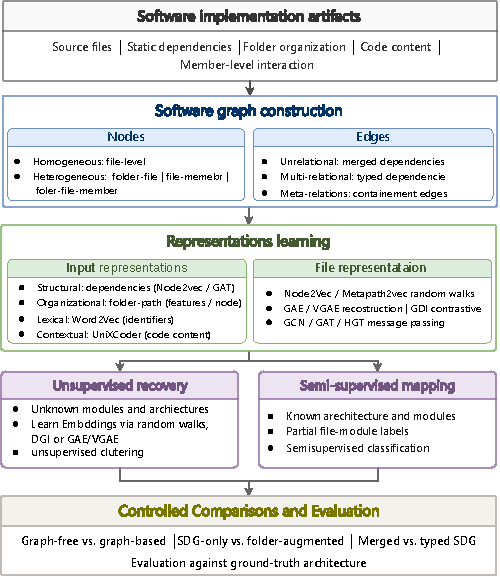
\includegraphics[width=1\textwidth]{figures/thesis_pipeline.pdf}
    \caption{Design space studied across the thesis. Software implementation artifacts are represented as graph configurations ranging from the homogeneous SDG to heterogeneous folder-file-member graphs. Structural, organizational, lexical, contextual, and interaction-level signals provide input representations, from which representation-learning methods derive file embeddings. These embeddings support unsupervised recovery and semi-supervised mapping and are evaluated against ground-truth reference decompositions. Across studies, controlled comparisons examine relation modeling, graph structure, input representations, and graph-based learning.}
    % \caption[Design space studied in the thesis.]{Design space studied across the thesis: graph configurations ranging from the SDG to heterogeneous folder-file-member graphs, initialized from structural, organizational, lexical, or contextual signals, and evaluated under unsupervised recovery and semi-supervised mapping through controlled comparisons of relation modeling, graph structure, input signal, and message passing itself.}
    % \label{fig:design_space}
\end{figure}

\subsection{Research Trajectory \label{sec:research_traj}}

The studies in this thesis form an incremental investigation of graph-based representation learning for architectural analysis, on the premise that architectural information is distributed across static dependencies, project organization, and source-code content. This framework integrates or isolates these sources: dependency relations define a file's structural context, while node and edge attributes encode organizational, lexical, contextual, or interaction-level information. Each study addresses limitations identified in the previous one, investigating how these sources should be represented and learned from, rather than assuming one graph construction, feature representation, or encoder is uniformly appropriate.

The prior graph-based representation learning approach to architecture recovery, NEGAR~\cite{negar}, learns file embeddings from SDG via node2vec-style random walks and clusters them into modules. It evaluates dependency types through separate pipelines and does not incorporate folder organization or lexical information. This leaves open whether typed dependencies can be modeled jointly and whether organizational and lexical signals provide complementary evidence for recovery. GAER~\cite{gaer} addresses this question by representing typed dependencies as relation-specific graph structures and combining folder paths and code identifiers as node features within a graph autoencoder framework. It further examines how encoder choice (GCN vs.\ GAT) and cluster granularity affect the results. However, because these signals are fused within the same configuration, the contribution of each source cannot be separated from the others.

A subsequent recovery study investigates a different self-supervised learning objective. It uses contrastive learning rather than graph reconstruction and augments file-level dependency edges with attributes that describe the member-level interactions that give rise to each dependency. This examines whether interaction type and frequency provide useful architectural information beyond the existence of a file-level dependency~\cite{arl_2026}. A further recovery study then examines dependency structure and project organization more directly. It compares dependency-only file graphs with folder-augmented heterogeneous graphs using both random-walk and graph-attention representation learners. The graph-attention variants are trained with a variational graph autoencoder, and the study additionally evaluates positional encoding~\cite{lpe} and diffusion-based structural augmentation~\cite{gdc} to extend the effective reach of shallow message-passing models~\cite{structsar}.

The remaining two studies turn to mapping source files to architectural modules, where the module set is known, and a subset of files is labeled. This study formulates mapping as semi-supervised node classification with iterative self-training over a multi-relational graph~\cite{mapping_ext}. It further introduces a graph-free multi-layer perceptron (MLP) baseline, trained under the same features and self-training procedure, to compare GNN-based prediction against feature-only prediction, a comparison absent from the recovery studies. The resulting difference indicates what the GNN encoder contributes beyond the file-level features, though it does not isolate message passing alone, since the models also differ in parameterization.

The final study extends this mapping design by introducing a dependency-guided contextual code representation and by expanding the graph to include folder and member nodes. It compares structural, lexical, and contextual representations both without message passing and as inputs to the same heterogeneous graph transformer, across graph variants that add or remove folder and member nodes. Thus, rather than directly validating all earlier results, it tests how these representations and graph structures contribute under one matched semi-supervised mapping setting.

% ============================================================
% Graph and Signal Representation
% Subsection 3 of 3 under Chapter 4, Section "Research Design"
%   (alongside: Design Space, Research Trajectory)
% ============================================================

\subsection{Graph and Signal Representation}
\label{sec:graph_signal_representation}

The design space defines the representational choices in the abstract. This subsection instantiates them concretely, showing which graph each study constructs and which signals it places on that graph's nodes and edges. Table~\ref{tab:graph_signal} summarizes both axes across the five studies; the prose that follows explains why each study sits where it does.

\subsubsection{Graph Construction}

The five studies construct their graphs at increasing levels of richness, each adding structure the previous studies could not represent. GAER and the architecture representation learning study model the system as a multi-relational, file-level SDG, keeping dependency types such as \emph{call}, \emph{import}, and \emph{inheritance} as separate, relation-specific edges; neither goes beyond file-level nodes. The controlled variational-GAE study isolates project organization from this file-level structure by comparing a single-relation SDG against the same graph augmented with folder nodes and folder--file containment relations, including a typed-dependency variant within that heterogeneous setting, to test whether organizational structure contributes beyond dependencies alone. The C2A mapping extension carries the multi-relational, file-level SDG into a supervised setting without extending its structure further. The heterogeneous graph study then adds member nodes that aggregate each file's methods and fields, connected by file--member containment alongside the existing folder--file containment and file--file dependency relations, reaching the finest granularity studied in this thesis.

\begin{table}[!t]
\caption{Graph construction and signal representation across the five studies. Edge attributes carry relation type only, except ARL-E, which adds interaction type and frequency, and StructSAR's diffusion variant, which attaches a personalized PageRank (PPR) edge weight.}
\label{tab:graph_signal}
\begin{threeparttable}
\begin{adjustbox}{max width=\textwidth}
\begin{tabular}{@{} l l l l @{}}
\toprule
\textbf{Study} & \textbf{Nodes} & \textbf{Dependencies} & \textbf{Node features} \\
\midrule
GAER & File & Multi-relational SDG & Path BoW $\Vert$ W2V ids \\
ARL / ARL-E & File & Multi-relational SDG & Path BoW $+$ id BoW \\
C2A mapping & File & Multi-relational SDG & Path BoW $\Vert$ W2V ids \\

\midrule
StructSAR& Folder, file & Single- or multi-relational & Learnable id ($+$LPE) \\
HetMap & Folder, file, member & Multi-relational & W2V / N2V / UniXcoder \\
\bottomrule
\end{tabular}
\end{adjustbox}
\begin{tablenotes}
\footnotesize
\item BoW = bag-of-words; W2V = Word2Vec; N2V = node2vec; LPE = Laplacian positional encoding.
\end{tablenotes}
\end{threeparttable}
\end{table}

\subsubsection{Input Signal Representation}

Node feature construction instantiates the feature axis of the design space at the study level. GAER and the C2A mapping extension initialize every file node from external signal, concatenating a binary file-path bag-of-words vector with an $\ell_2$-normalized average of Word2Vec embeddings over its code identifiers, so that organizational and lexical evidence enter the encoder together as one fixed input. The architecture representation learning study draws on the same two sources but encodes both as binary token vectors with $\ell_2$ normalization, using a bag-of-words encoding of identifiers in place of a separately trained lexical embedding. The controlled variational-GAE study uses no external node signal: each node type receives a learnable identity embedding trained with the model, and file nodes additionally carry a Laplacian positional encoding concatenated to that embedding, so the encoder is supplied with position in the dependency graph rather than folder or lexical content. Its random-walk baselines are a further case with no node feature vector at all, since node2vec and MetaPath2Vec learn embeddings directly from walk co-occurrence over the graph.

The heterogeneous graph study treats node initialization as the object of study rather than a fixed choice. It compares three external strategies for file and member nodes under otherwise matched conditions: lexical Word2Vec embeddings over identifiers, structural node2vec embeddings over the dependency graph, and contextual UniXcoder embeddings in both zero-shot and dependency-guided fine-tuned form. Folder nodes, when present, are always encoded from binary folder-path tokens irrespective of the strategy used for file and member nodes, keeping the organizational signal fixed while the file- and member-level representation varies.

Edge attributes form a narrower axis, extended beyond relation type in only two of the five studies; elsewhere edges carry their type alone and all relational evidence passes through multi-relational message passing. The architecture representation learning study augments its file-level edges with an attribute vector describing how each dependency arises, concatenating a binary, $\ell_2$-normalized encoding of the member-level interaction type that produced the dependency with a log-normalized count of how often that interaction occurs between the two files, testing whether the origin and frequency of a dependency add information beyond the presence of a typed edge. The controlled variational-GAE study attaches an edge attribute of a different nature in its diffusion variant, where graph diffusion convolution rewires the file graph through Personalized PageRank and gives each rewired edge a scalar weight that biases the attention logits toward diffusion-close neighbors. That weight is an artifact of the diffusion process rather than external content of the kind folder, lexical, and contextual features supply, so edge attribute initialization does not constitute a third input axis co-equal with node features. It is a targeted extension, used where a study's question concerns interaction semantics or the reach of shallow message passing.

\section{Learning Settings}
\label{sec:method-learning}

The two tasks are studied under different learning settings, and the settings answer related but not identical questions. Unsupervised recovery has no labels to train against, so a graph autoencoder or its variational form reconstructs observed graph structure from the learned representations, or a contrastive objective such as deep graph infomax trains the encoder by distinguishing the observed graph from a corrupted view, and the resulting file embeddings are clustered into modules after training. The number of modules is itself unknown and is searched over rather than fixed, so a recovery result is a partition whose granularity the method itself must choose. Semi-supervised mapping has a target module set that is known in advance and a small initial labeled set, so a classifier, built on a graph convolution, attention, or heterogeneous transformer encoder, predicts module membership directly, and the labeled set is expanded through iterative self-training as the model's own confident predictions are added back into the training data.

Clustering and classification are evaluated with different metrics for this reason, not only by convention. A clustering agreement measure such as the adjusted Rand index rewards a partition for resembling the reference regardless of how many clusters it contains, since the method was never told how many modules to produce, while a classification metric such as macro-F1 evaluates predictions against a fixed, known label set that the method receives as part of its supervision. This is why recovery and mapping results are never merged into one pooled statistic anywhere in this thesis: an improvement in ARI and an improvement in macro-F1 are answers to related but structurally different questions, and treating them as interchangeable would misstate what each setting can show.

\section{Controlled-Comparison Logic}
\label{sec:method-comparison}

The design space is not searched by optimizing over its dimensions jointly, which is the strategy this thesis positions itself against, since fixed weightings tuned once do not adapt across systems. It is searched by controlled comparison: within a study, one dimension is varied while the others are held fixed, so that a difference in outcome can be attributed to that dimension rather than to a confounded change elsewhere. Three instances of this logic carry most of the thesis's evidence. A graph-free multi-layer perceptron, trained on the same features and the same self-training loop as its graph-based counterparts, is compared against them in the mapping studies; because the only difference between the models is the presence of message passing, any systematic gap is attributable to the dependency graph itself, which is why this comparison is the strongest available evidence for what the graph contributes beyond the features already present at each file. A dependency-only graph is compared against the same graph augmented with folder nodes, with the encoder and training objective held fixed, which is why this comparison, rather than a comparison between two different encoders or two different systems, is what tests the contribution of organizational structure specifically. HetMap's design combines both principles at once: it varies the file's feature initialization and the graph structure independently of each other, so that a result can be attributed to the feature, to the graph, or to their interaction rather than to a single confounded change, which is why it is treated as the strongest evidence in the thesis for whether two signals are complementary or redundant.

Whether a design choice is justified is decided by paired comparison rather than by a single point estimate, and the specifics of that comparison are stated in Section~\ref{sec:method-evaluation}. The studies do not sample the design space independently of one another, as Section~\ref{sec:method-cumulative} already established, so the consequence of this logic is that this is not a fully crossed factorial design, and it is not presented as one. It is a set of overlapping controlled comparisons that share a benchmark of systems and a common criterion for what counts as a benefit, each isolating one or two dimensions, with the richest study returning to re-test earlier conclusions once several signals are available within a single model.

\section{Subjects, Ground Truth, and Evaluation Protocol}
\label{sec:data}

The studies in this thesis are run on open-source systems drawn from published software architecture recovery and code-to-architecture mapping research, summarized in Table~\ref{table:dataset_details_unified}. For each system, the table records the properties the studies read their results against: the number of modules in the reference architecture, the number of files and static dependencies, the average node degree, and the homophily of the dependency graph with respect to the reference modules. The systems span three languages and a wide range of size and structure, from small single-purpose libraries to Chromium at several million lines, which is what lets the conditions under which a design choice helps be observed rather than assumed. Not every study uses the full set; each draws the subset appropriate to its setting, and the individual papers state the exact selection and its provenance.

\begin{table}[htb]
\centering
\caption[Benchmark systems properties and version.]{\small Properties and versions of studied software systems. $\mathcal{C}$ denotes modules in the GT architecture, SD are the static dependencies between files, and the average node degree is computed as $\langle k \rangle = |\text{SD}|/|\text{Files}|$. \label{table:dataset_details_unified}}
\renewcommand{\arraystretch}{1.05}
\small
\begin{adjustbox}{max width=\columnwidth}
\begin{tabular}{c l l r r r r c c l}
\toprule
& System
& Version
& LoC
& $|\mathcal{C}|$
& $|\text{Files}|$
& $\boldsymbol{|\text{SD}|}$
& $\mathcal{H}$
& $\langle k \rangle$
& Domain\\
\midrule
\multirow{10}{*}{\rotatebox[origin=c]{90}{Java}}
& \href{https://ant.apache.org/}{Ant}
& r584500  & 36k & 15 & 815  & 12\,028  & 0.37 & 14.8 & Process automation \\
&\href{https://github.com/isr-uci-edu/ArchStudio4}{ArchStudio4}
& 4  & 280K & 57 & 583 & 5418 & 0.67 & 9.3 & Architecture modeling \\
& \href{http://argouml.tigris.org/}{ArgoUML}
& r13713   & 62k & 14 & 766    & 9\,491   & 0.54 & 12.4 & UML modeling\\
& \href{https://commons.apache.org/proper/commons-imaging/}{C.Img}
& v1.0a2   & 18k & 21 & 329    & 4\,561   & 0.61 & 13.9 & Image I/O library\\
&\href{https://github.com/isr-uci-edu/ArchStudio4}{Hadoop}
& 0.19.0 & 200K & 67 & 591 & 10\,510 & 0.34 & 17.8 & Distributed processing \\
& \href{https://jabref.org/}{JabRef}
& v3.7     & 59k & 6  & 1\,180  & 17\,557  & 0.58 & 14.9 & Reference management \\
& \href{https://lucene.apache.org/}{Lucene}
& r1075001 & 36k & 7  & 1\,054  & 18\,595  & 0.68 & 17.6 & Search engine \\
&\href{https://oodt.apache.org/}{OODT}
& 0.2      & 180K    & 216  & 876   & 8811 & 0.26 & 10.1 & Data management \\
& \href{https://www.sweethome3d.com/}{SH-3D}
& r002382  & 35k & 9  & 191  & 3912   & 0.34 & 20.5 & Interior design \\
& \href{https://TeamMatesv4.appspot.com/web/front/home}{TeamMates}
& v5.11    & 55k & 15 & 778    & 17\,818  & 0.33 & 22.9 & Peer feedback system \\
\midrule
\multirow{3}{*}{\rotatebox[origin=c]{90}{C}}
& \href{https://www.gnu.org/software/bash/}{Bash}
& 4.2      & 115k & 14 & 292    & 1\,222   & 0.60 & 4.2 & Shell \\
& \href{https://gitee.com/openharmony/drivers_framework}{HDF}
& 0e196f   & 153k & 9  & 153    & 1\,220   & 0.35 & 8.0 & Driver subsystem \\
&\href{https://gitlab.gnome.org/GNOME/Libxml}{Libxml}
& 2.4.22 & 81K & 17 & 82 & 986 & 0.21 & 12.0 & XML parser\\
\midrule
\multirow{2}{*}{\rotatebox[origin=c]{90}{C++}}
& \href{https://www.chromium.org/}{Chromium}
& svn-171054 & 11M & 69 & 18\,343 & 284\,435 & 0.58 & 15.5 & Web browser \\
& \href{https://gitee.com/openharmony/distributed_camera}{HDC}
& 46ff87   & 26k  & 11 & 207    & 1\,117   & 0.63 & 5.4 & Camera interface \\
\bottomrule
\end{tabular}
\end{adjustbox}
\end{table}

The reference (ground-truth) decompositions were not produced for this thesis. They come from expert-validated benchmarks contributed by the systems' own developers, by industry partners, or by researchers reconstructing a decomposition from documentation and code inspection~\cite{garcia2013,olsson2022automatically,Brunet_gt,lenhard2019exploring,sarif,olsson2021s4rdm3x}, and are reused here so that results remain directly comparable with prior baselines evaluated on the same systems and so that no new judgment enters the evaluation.

A reference decomposition of this kind is a judgment rather than a measurement. Files that plausibly belong to more than one module are resolved differently by different annotators, and reasonable experts disagree on where architectural boundaries fall. A recovery or mapping that departs from the reference is therefore not necessarily wrong, and a method that matches it on every system is not right in a stronger sense than the reference itself. The metrics are read in this light throughout the thesis.

Metric definitions are given once, in Section~\ref{sec:bg-eval}, and are not repeated here. What is stated here is how those metrics are applied across every controlled comparison in the thesis. Because both the initial labeled set and neural training introduce stochastic variation, each configuration is run one hundred times, and the configurations being compared in a given ablation share the same random seed and the same initial conditions on each run, so that a run of one configuration is matched to a run of the other rather than compared across independently drawn samples. Central tendency is summarized by the median across runs, which is less sensitive to outlying runs than the mean, and differences are assessed for statistical significance using the Wilcoxon signed-rank test on paired runs, reported together with Cliff's delta as an effect size using the standard negligible, small, medium, and large convention, with $p$-values Holm-corrected within each family of comparisons to control for the number of tests performed. Results are reported per system rather than averaged across systems, since averaging a metric across systems with different properties can cancel effects that act in opposite directions and obscure exactly the conditioning that the research questions ask about.

\section{Threats Addressed by Design}
\label{sec:method-threats}

Six threats recur across the studies, and the design choices already described in this chapter are, in each case, a direct response to one of them rather than an afterthought.

Metric dependence is addressed by never relying on a single score. A2A remains uniformly high across methods and systems and therefore separates methods poorly on its own; \cc{} is sensitive to a fixed coverage threshold and can drop sharply from a single split reference module; macro-F1 is sensitive to skewed module sizes, so a difference on a system with one dominant module is read alongside micro-F1 rather than in isolation. The recovery studies report a battery of complementary metrics for this reason, and the mapping studies report both macro- and micro-F1 throughout.

Ground-truth subjectivity is addressed by using only published, expert-validated mappings and constructing none for this thesis, as stated in Section~\ref{sec:data}, and by treating a departure from the reference as evidence to be interpreted rather than as an error to be corrected.

Folder-reference correspondence is a confound specific to organizational signal. Where a system's architecture was defined by its own developers, folder layout and the reference decomposition reflect the same organizational decisions, and where the architecture was reconstructed by researchers, folder structure was itself one of the cues that reconstruction used. Folder location can therefore align with the reference for reasons unrelated to its standing as an independent architectural signal. This thesis addresses the threat by design rather than by disclaimer alone: the dependency-only versus folder-augmented comparison in Part~I and the feature-versus-graph variation in HetMap make it possible to state how much of folder structure's apparent strength survives when it is isolated from, or removed alongside, the other signals.

Static dependency extraction error is addressed by verification rather than by assumption. Where dependencies could not be reliably extracted for a candidate system and prior baseline results could not be reproduced on it, the system was dropped from the study rather than retained with an unreliable graph.

Stochasticity from random initialization and neural training is addressed by the evaluation protocol of Section~\ref{sec:data} directly: repeated runs, paired comparison under shared seeds, median reporting, and effect sizes read alongside Holm-corrected significance, since with a hundred runs per configuration a test can detect systematic differences that are statistically real but practically small, and effect size is what distinguishes the two.

Cross-system heterogeneity, the fifteen systems spanning three languages and several orders of magnitude in size, is treated as an asset rather than only a threat once results are never pooled across systems and are instead read against the measured properties of Table~\ref{table:dataset_details_unified}, homophily, connectivity, and module count, so that a finding is stated together with the conditions under which it holds rather than as a claim assumed to transfer to every system in the benchmark.
\cleardoublepage

% % ---------------------------------------------------------------------
% CHAPTER — SYNTHESIS
% Working draft. Prose states the conditioned-answer structure of each RQ.
% "% INSERT" markers show where a specific result / effect size is slotted
% from the named study, so no quantity is asserted here before its chapter
% reports it.
% ---------------------------------------------------------------------
\chapter{Synthesis}
\label{ch:synthesis}
 \chaptertoc
 
This chapter returns to the three research questions of Section~\ref{sec:research-objectives} and states the answer each receives once the studies are read together. The answers are read off the controlled comparisons of Chapter~\ref{ch:methodology}: each study isolates one part of the design space, and the synthesis is what those isolated comparisons say in combination, against the system properties recorded in Table~\ref{table:dataset_details_unified}. None of the three questions resolves to a single ranking of methods. Each resolves to a design choice or a signal together with the conditions under which it carries architectural information, and it is the conditioning, not the ranking, that transfers across systems and across the two tasks.
 
\section{RQ1: Which Design Choices Are Justified}
\label{sec:syn-rq1}
 
RQ1 asks which choices of graph granularity, relation modeling, encoder, and learning objective are justified by measurable benefit. Read across the studies, the answer is that the benefit of a choice is decided by the graph it operates on rather than by the choice in isolation, and the studies make this concrete one axis at a time.
 
The comparison of degree-normalized convolution with attention illustrates the point. In supervised mapping, attention is the stronger and safer default: the relation-typed attention encoder is the best-performing learned model, whereas the convolutional encoder does not consistently improve on the graph-free baseline, and the depth at which it is useful depends on the granularity, connectivity, and homophily of the system rather than being fixed. % INSERT: C2A ICSA main results (GAT best; GCN not consistently > MLP) + depth ablation effect sizes; state the systems where GCN depth helps vs hurts.
The recovery studies compare the same two encoders within the reconstruction framework, where the decision is made without labels. % INSERT: GAER GCN vs GAT verdict + the condition under which one is preferred; note granularity (number of clusters) effect.
 
Keeping dependency types apart through relation-specific parameters, rather than collapsing them into a single weighted graph, is justified where the types carry distinct architectural meaning and does not pay for itself where they do not. % INSERT: C2A typed-vs-collapsed and edge-direction result; GAER heterogeneous-encoder motivation and any type-specific gain.
The learning objective is the axis particular to unsupervised recovery, where a reconstruction objective and a contrastive objective are available in the absence of labels. % INSERT: ARL (contrastive) vs GAER (reconstruction) comparison and the condition that separates them.
 
The richest representation extends the graph itself, from a file-only graph to one that adds folder and member-level nodes, processed by a meta-relation attention encoder. Whether this added structure is justified is not settled at the level of the encoder but at the level of what the extra nodes contribute, which is the subject of RQ3. % INSERT: HetMap HGT vs GAT/MLP headline (RQ1 table) — state where the heterogeneous representation wins and where it does not.
 
\section{RQ2: What Each Input Signal Carries}
\label{sec:syn-rq2}
 
RQ2 asks what architectural information dependency structure, project organization, and code identifiers carry, and under which system properties each is reliable. The answer is stated per signal, and each signal's reliability is tied to a property that Table~\ref{table:dataset_details_unified} records or that the studies measure, so that the claim is conditional rather than general.
 
The contribution of the dependency graph is isolated by the graph-free baseline, which predicts module assignments from node features alone under the same training procedure. What the graph adds over the features is therefore measured directly rather than inferred. % INSERT: C2A ICSA RQ2 result — graph contribution beyond features, and its dependence on homophily / dependency cohesion (name the systems where the graph helps and where it does not). Coverage effect (MLP maps ~60% at 0.95 confidence vs ~97% with the graph) belongs here.
Read against homophily, the dependency signal is informative where dependencies concentrate within reference modules and weak where cross-module coupling, for example through widely used utility code, dominates the local neighborhood.
 
Project organization enters as folder structure, and its reliability tracks how closely the folder hierarchy aligns with the reference decomposition. Where that alignment is high, folder structure is a strong architectural proxy and can carry much of the result on its own; where it is low, it is noise, since utility directories mix entities from several modules. % INSERT: GAER dependency-only vs folder-augmented comparison; StructSAR folder-organization result. The "shown by removing it" ablation for directory structure (contribution C4) is stated here.
Code identifiers carry domain vocabulary that aligns with module membership where the vocabulary is separable across modules, and they blur where the same terms recur across modules. % INSERT: ARL lexical-signal result; HetMap file-feature (Word2Vec / node2vec) behavior as it bears on lexical vs structural initialization.
 
\section{RQ3: How Signals Interact in a Richer Graph}
\label{sec:syn-rq3}
 
RQ3 asks how the usefulness of structural, lexical, and contextual file representations changes once they are available together within a heterogeneous graph, and where the sources are complementary rather than redundant. It is answered principally by the capstone study, which varies file representation and graph structure independently while holding the learning setting fixed, and it functions as a test of whether the RQ1 and RQ2 conclusions survive once the signals are combined.
 
The distinction the study draws is between a gain that reflects new architectural evidence and a gain that reflects a signal already aligned with the reference. Adding member-level structure to the folder-file graph improves mapping where the added interactions separate files that the coarser graph confused, and does not improve it where folder organization has already saturated the achievable performance. % INSERT: HetMap RQ3 significance table (F vs MLP, FM vs MLP, FM vs F) read by system; name the systems where member structure adds (complementary) and where folder alignment saturates (redundant).
The interaction also depends on how the file node is initialized. A lexical initialization and a structural, random-walk initialization respond differently to the same added graph structure, because a representation that already encodes neighborhood structure has less to gain, and can lose, from further message passing over that structure. % INSERT: HetMap Word2Vec vs node2vec contrast from the RQ3 table — state where message passing helps the lexical init and where it is neutral or harmful for the structural init.
 
The consequence for the thesis is that the value of a signal is not additive. A signal that is informative in isolation, as established under RQ2, can be redundant once another aligned signal is present, and the heterogeneous model makes this visible rather than hiding it inside an aggregate score.
 
\section{Consolidated Contributions}
\label{sec:syn-contributions}
 
The three conditioned answers restate the contributions claimed in Chapter~\ref{ch:introduction}. That learned representations outperform hand-tuned fusion, most clearly at the scale where fixed weightings are most brittle, is the combined verdict of RQ1 and RQ2 across the two tasks. The isolation of what each signal contributes and where it fails is the substance of RQ2. That the same design choices and signals behave consistently across unsupervised recovery and supervised mapping, which no single study can claim, is what the shared design space of Chapter~\ref{ch:methodology} makes demonstrable. And that directory structure is a strong architectural proxy, shown by removing it rather than by asserting it, is the specific result folded into RQ2.
% \cleardoublepage



%------------------------------------------------------------------
%---------------------Refrences & Appendix ------------------------
%------------------------------------------------------------------
\phantomsection
\addcontentsline{toc}{chapter}{Bibliography}
\renewcommand*{\bibfont}{\small}
\printbibliography

% \begin{appendices}
%\appendixpage
\noappendicestocpagenum
\addappheadtotoc


\renewcommand{\myfullcite}[1]{\printpublication{#1}.}



\renewcommand{\appendixname}{Paper}
\chapter{A changeset-based approach to assess source code density and developer efficacy}\label{app:publ-honel2018changeset}
\chaptermark{\label{app:publ-honel2018changeset}}
\myfullcite{honel2018changeset}

\vspace{10pt}
\noindent
{\footnotesize Reprinted under the ACM reuse author rights.}
\includepdf[pages=-,pagecommand={},addtotoc={
  1,section,1,Introduction,p1_1, 
  1,section,1,Research Gap,p1_2,
  2,section,1,Method,p1_3,
  2,section,1,Results and Discussion,p1_4,
  2,section,1,Conclusion and Future Work,p1_5,
  2,section,1,References,p1_6}
]{papers/A_ICSE18_print.pdf}



\chapter{Importance and Aptitude of Source Code Density for Commit Classification into Maintenance Activities}\label{app:publ-honel19importance}
\chaptermark{\label{app:publ-honel19importance}}
\myfullcite{honel19importance}

\vspace{10pt}
\noindent
{\footnotesize\copyright~2019~{IEEE}. Reprinted, with permission.}
\includepdf[pages=-,pagecommand={},addtotoc={
   1,section,1,Introduction,p2_1,
   2,section,1,State Of the Art,p2_2,
   2,section,1,Methodology,p2_3,
   6,section,1,Results,p2_4,
  11,section,1,Threats to Validity,p2_5,
  11,section,1,Conclusions,p2_6,
  12,section,1,Future Work,p2_7,
  12,section,1,References,p2_8}
]{papers/B_QRS19_print.pdf}



\renewcommand{\appendixname}{Article}
\chapter{Using source code density to improve the accuracy of automatic commit classification into maintenance activities}\label{app:publ-honel2020using}
\chaptermark{\label{app:publ-honel2020using}}
\myfullcite{honel2020using}

\vspace{10pt}
\noindent
{\footnotesize Reprinted under the Elsevier reuse author rights.}
\includepdf[pages=-,pagecommand={},addtotoc={
   1,section,1,Introduction,p3_1,
   2,section,1,Background,p3_2,
   4,section,1,Methodology,p3_3,
   7,section,1,Results,p3_4,
  14,section,1,Threats to Validity,p3_5,
  15,section,1,Related Work,p3_6,
  16,section,1,Conclusions,p3_7,
  17,section,1,Future Work,p3_8,
  18,section,1,References,p3_9}
]{papers/C_JSS20_print.pdf}



\renewcommand{\appendixname}{Paper}
\chapter{Exploiting Relations, Sojourn-Times, and Joint Conditional Probabilities for Automated Commit Classification}\label{app:publ-honel2023hmm}
\chaptermark{\label{app:publ-honel2023hmm}}
\myfullcite{honel2023hmm}

\vspace{10pt}
\noindent
{\footnotesize Reprinted, with permission from {SciTePress}.}
\includepdf[pages=-,pagecommand={},addtotoc={
   1,section,1,Introduction,p4_1,
   2,section,1,Problem Statement,p4_2,
   4,section,1,Background,p4_3,
   6,section,1,Method,p4_4,
   7,section,1,Empirical Evaluation,p4_5,
   8,section,1,Summary and Conclusions,p4_6,
   8,section,1,References,p4_7}
]{papers/D_ICSOFT23_print.pdf}



\chapter{\texorpdfstring{Process Anti-Pattern Detection\,--\,a Case Study}{Process Anti-Pattern Detection - a Case Study}}\label{app:publ-picha_honel22pilot}
\chaptermark{\label{app:publ-picha_honel22pilot}}
\myfullcite{picha_honel22pilot}

\vspace{10pt}
\noindent
{\footnotesize Reprinted under the ACM reuse author rights.}
\includepdf[pages=-,pagecommand={},addtotoc={
   1,section,1,Introduction,p5_1,
   2,section,1,Related Work,p5_2,
   3,section,1,Study Design,p5_3,
   6,section,1,Study Execution,p5_4,
  10,section,1,Results,p5_5,
  11,section,1,Discussion of the Case Study,p5_6,
  16,section,1,Conclusions,p5_7,
  17,section,1,References,p5_8}
]{papers/E_EuroPLOP22_print.pdf}



\renewcommand{\appendixname}{Article}
\chapter{Activity-Based Detection of (Anti-)Patterns: An Embedded Case Study of the Fire Drill}\label{app:publ-honel2023embedded}
\chaptermark{\label{app:publ-honel2023embedded}}
\myfullcite{honel2023embedded}

\vspace{10pt}
\noindent
{\footnotesize Reprinted under the Creative Commons Attribution 4.0 International license.}
\includepdf[pages=-,pagecommand={},addtotoc={
   1,section,1,Introduction,p6_1,
   5,section,1,Related Work,p6_2,
   7,section,1,Background,p6_3,
   9,section,1,Case Study Design,p6_4,
  21,section,1,Analysis and Results,p6_5,
  30,section,1,Discussion,p6_6,
  32,section,1,Conclusions - Synthesis,p6_7,
  33,section,1,References,p6_8,
  39,section,1,Appendix,p6_9}
]{papers/F_EINF23_print.pdf}



\renewcommand{\appendixname}{Paper}
\chapter{Contextual Operationalization of Metrics as Scores: Is My Metric Value Good?}\label{app:publ-honel2022qrsmas}
\chaptermark{\label{app:publ-honel2022qrsmas}}
\myfullcite{honel2022qrsmas}

\vspace{10pt}
\noindent
{\footnotesize\copyright~2022~{IEEE}. Reprinted, with permission.}
\includepdf[pages=-,pagecommand={},addtotoc={
   1,section,1,Introduction,p7_1,
   2,section,1,Background,p7_2,
   3,section,1,Research Design,p7_3,
   4,section,1,Application: Metrics As Scores,p7_4,
   6,section,1,Results,p7_5,
   8,section,1,Discussion,p7_6,
  10,section,1,Threats to Validity,p7_7,
  10,section,1,Related work,p7_8,
  10,section,1,Future Work,p7_9,
  11,section,1,References,p7_10}
]{papers/G_QRS22_print.pdf}



\renewcommand{\appendixname}{Article}
\chapter{Metrics As Scores: A Tool- and Analysis Suite and Interactive Application for Exploring Context-Dependent Distributions}\label{app:publ-honel2023masjoss}
\chaptermark{\label{app:publ-honel2023masjoss}}
\myfullcite{honel2023masjoss}

\vspace{10pt}
\noindent
{\footnotesize Reprinted under the Creative Commons Attribution 4.0 International license.}
\includepdf[pages=-,pagecommand={},addtotoc={
   1,section,1,Summary,p8_1,
   2,section,1,Statement Of Need,p8_2,
   2,section,1,MAS - The Tool- and Analysis Suite,p8_3,
   3,section,1,MAS - The Interactive Application,p8_4,
   4,section,1,Applications,p8_5,
   4,section,1,Related Work,p8_6,
   4,section,1,References,p8_7}
]{papers/H_JOSS23_print.pdf}



\end{appendices}
% \cleardoublepage
% \cleardoublepage
% \backmatter
% \cleardoublepage
\end{document}